\chapter{Worm Model}
\label{chap:worm}

\begin{figure}[tb] 
  \centerline{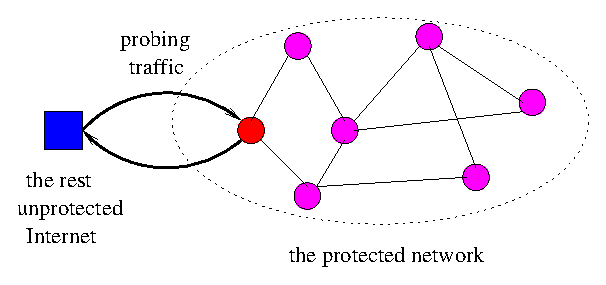
\includegraphics [width=3in] {dn-an.eps}}
  \caption{\small The DN-AN model.}
  \label{fig:dn-an}
\end{figure}

In this chapter,
  we describe a scalable worm propagation model in~\ns,
  namely the detailed-network and abstract-network (DN-AN) model.
It combines packet-level simulations with analytic worm spreading model.
As shown in Figure~\ref{fig:dn-an},
  we model the Internet with two parts: detailed, and abstract part.
A detailed-network could be an enterprise-network or the network run by an ISP.
It simulates network connectivity and packet transmission.
Users can evaluate worm detection algorithms in the detailed network.
On the other hand,
  we abstract the rest of the Internet with a mathematical model,
  namely susceptible-infectious-removal (SIR) model
  (refer to~\cite{Hethcote00inf} for detailed descriptions).
Compared to the detailed network,
  we only track several state variables in the abstract world,
  such as the number of infected hosts.
The interaction between DN and AN is through actual packet transmissions,
  that is, the probing traffic generated by compromised hosts in
  both parts.

For detailed description on DN-AN model,
  please refer to our draft paper.
We implement the worm propagation model as applications.
The source code can be found at \nsf{/apps/worm.\{cc,h\}}.
There is also a sample script to illustrate the DN-AN model under
  \nsf{/tcl/ex/worm.tcl}.

\section{Overview}
\label{sec:worm:overview}

We implement the worm propagation model with three classes:
  \clsref{WormApp, DnhWormApp, and AnWormApp}{ns-2/apps/worm.\{cc,h\}}. 
\clsref{WormApp} and \clsref{DnhWormApp} are used in the detailed network,
  representing invulnerable and vulnerable hosts respectively.
\clsref{AnWormApp} is the abstract network.
Currently,
  our model only supports UDP-based worms.

An vulnerable host is compromised upon receiving a probing packet.
Then,
  it chooses a target host (randomly or with certain preference to local
  neighbors) to scan.
Probing packets have no effect on invulnerable hosts.
When the abstract network receives probing packets,
  it updates its current states.

\section{Configuration}
\label{sec:worm:config}

To set up simulation scenario,
  we first build the detailed network.
We also need to create one extra node to represent the abstract network, 
  and connect it to the detailed network.

For nodes in the detailed network,
  we first attach a \code{MessagePassing} agent to each node:

\begin{program}
  set a [new Agent/MessagePassing]
  $n attach $a $probing_port
\end{program}

If the node represents a vulnerable host,
  we use \clsref{DnhWormApp}:

\begin{program}
  set w [new Application/Worm/Dnh]
  $w attach-agent $a
\end{program}

Otherwise, we configure the node as invulnerable:
\begin{program}
  set w [new Application/Worm]
  $w attach-agent $a
\end{program}


We configure the abstract network as:

\begin{program}
  set a [new Agent/MessagePassing]
  $na attach $a $probing_port
  set w [new Application/Worm/An]
  $w attach-agent $a
\end{program}

In order for the abstract network to receive probing packets generated by
  nodes within the detailed networks,
  we need to use manual routing.
There are some extra configuration for the abstract-network node:

\begin{program}
  set p [$na set dmux_]
  $p defaulttarget $a
  [$na entry] defaulttarget $p
\end{program}


\section{Commands at a glance}
\label{sec:worm:command}

Some common parameters can be configured through TCL script:
\begin{program}
  ScanRate    # the rate that a compromised host sends probing packets
  ScanPort    # the vulnerable service port number
  ScanPacketSize  # the size of worm probing packets
\end{program}

By default,
  compromised hosts scan the Internet randomly.
We can also simulate local-scanning worm by setting the local-scanning
  probability:
\begin{program}
  $w local-p 0.5    
\end{program}


Following are some commands to configure parameters for the
  abstract network:

\begin{program}
  $w beta 0.1   # infection parameter
  $w gamma 0   # removal parameter
  $w addr-range 2000 200000  # the address space of the abstract network
  $w dn-range 0 1999         # the address space of the detailed network
  $w v_percent 0.01          # the percentage of vulnerable hosts in the abstract network
\end{program}

